\documentclass{article}

\usepackage[utf8]{inputenc}
\usepackage[T1]{fontenc}
\usepackage{amsmath,amssymb,amsfonts}
\usepackage{graphicx}
\usepackage{booktabs}
\usepackage{hyperref}
\usepackage{xcolor}
\usepackage{geometry}
\usepackage{natbib}
\usepackage{tikz}
\usetikzlibrary{positioning, arrows.meta, shapes.geometric, fit, calc}

\geometry{margin=1in}

\title{Encoding and Gradient in Physics-Informed Networks: Tokenizer-Free Models and Controllable Explosion Optimization}

\author{Hengbo Li\\
\texttt{1147502779@qq.com}
}

\date{May 2026}

\begin{document}

\maketitle

\begin{abstract}
We present two analyses of training dynamics in physics-informed neural networks. First, we analyze tokenizer-free language models, comparing byte-level (UTF-8) and Unicode BMP encoding schemes. Unicode BMP reduces Chinese sequence length by 3x compared to UTF-8 bytes while preserving semantic completeness. We identify the collapse phenomenon in deep networks trained from scratch without pretraining, where both LSH-SFA~\cite{lsh-sfa} and Transformer baselines exhibit training instability, revealing this as a shared limitation of fine-grained byte-level classification rather than an architecture-specific defect. Second, we analyze the controllable explosion phenomenon in LSH-SFA, where gradient magnitudes explode exponentially during training (e.g., L0 loss increases from 1990 to $4.05 \times 10^{12}$) while the model converges robustly. We explain this through three mechanisms: (1) the conjugate Laplacian operator ensures gradient propagation direction aligns with energy descent; (2) inter-layer coupling coefficients decay progressively ($1.0 \rightarrow 0.8 \rightarrow 0.8 \rightarrow 0.8$); (3) energy conservation constraints in physical operators prevent divergence. We propose the V2 stateless gradient architecture and demonstrate 46.1\% loss reduction vs.\ 42.7\% for pure Autograd.
\end{abstract}

\section{Introduction}

Training dynamics in physics-informed neural networks differ fundamentally from standard architectures. This paper examines two aspects: the encoding scheme's impact on training stability, and the gradient behavior during convergence.

\subsection{The Encoding Problem}

Standard language models use subword tokenizers (BPE, WordPiece) that introduce language-specific biases and require separate training. Tokenizer-free models operate directly on bytes or Unicode code points, but face challenges:
\begin{itemize}
\item UTF-8 bytes expand Chinese text 3x, increasing sequence length
\item Fine-grained classification (256 or 65,536 classes) without pretraining leads to collapse
\item The relationship between encoding granularity and model capacity is poorly understood
\end{itemize}

\subsection{The Gradient Explosion Problem}

In LSH-SFA, gradient magnitudes can explode exponentially during training while the model still converges. This ``controllable explosion'' is counter-intuitive from a standard deep learning perspective, where gradient explosion typically leads to divergence. Understanding this phenomenon is critical for training stability.

\section{Part I: Tokenizer-Free Encoding}

\subsection{Encoding Schemes}

\subsubsection{UTF-8 Byte Level}

\begin{verbatim}
"中" -> [228, 184, 173]  # 3 tokens
\end{verbatim}

Problem: 3x sequence length for Chinese.

\subsubsection{Unicode BMP Level}

\begin{verbatim}
"中" -> [20013]  # 1 token
\end{verbatim}

Advantage: Direct semantic mapping, 3x reduction for Chinese.

\subsection{Collapse Phenomenon}

Both LSH-SFA and Transformer exhibit collapse in 4-layer models trained from scratch:

\begin{table}[h]
\centering
\caption{Collapse in deep models without pretraining.}
\label{tab:collapse}
\begin{tabular}{lccc}
\toprule
\textbf{Model} & \textbf{Layers} & \textbf{SST-2 Accuracy} \\
\midrule
LSH-SFA & 1 & 59.3\% \\
LSH-SFA & 4 & 50.9\% (collapse) \\
Transformer & 4 & 26.3\% (collapse) \\
\bottomrule
\end{tabular}
\end{table}

\textbf{Root cause analysis.} The collapse phenomenon arises from the combination of fine-grained output classification (256 or 65,536 classes) and the absence of pretraining. Without pretrained embeddings, the model must simultaneously learn both character-level representations and higher-level semantic patterns, creating conflicting gradient signals that destabilize training. Notably, LSH-SFA collapses less severely than the Transformer (50.9\% vs.\ 26.3\%), suggesting that physical priors provide partial regularization.

\subsection{Model Capacity Analysis}

\begin{table}[h]
\centering
\caption{Encoding scheme comparison.}
\label{tab:encoding}
\begin{tabular}{lcccc}
\toprule
\textbf{Scheme} & \textbf{Vocabulary} & \textbf{Chinese Len} & \textbf{Tokenizer-Free} \\
\midrule
UTF-8 Byte & 256 & 3x & Yes \\
BBPE & 50k+ & 1x & No \\
WordPiece & 30k & 1x & No \\
Unicode BMP & 65,536 & 1x & Yes \\
\bottomrule
\end{tabular}
\end{table}

Unicode BMP provides optimal balance: tokenizer-free operation, 1x Chinese sequence length, and a manageable vocabulary of 65,536 code points.

\section{Part II: Controllable Explosion Optimization}

\subsection{Observation}

During LSH-SFA training, gradient magnitudes explode exponentially:

\begin{verbatim}
Step 0:   L0=1990.14    L1=213.97    L2=20.50   L3=1.83
Step 400: L0=4.05e12    L1=1.25e9    L2=295248  L3=52.82
\end{verbatim}

Yet loss decreases from 46.56 to 17.77 (61.8\% reduction). The gradient explosion is \emph{controllable}: it does not prevent convergence.

\subsection{Theoretical Analysis}

\subsubsection{Mechanism 1: Conjugate Laplacian}

The Laplacian operator in the diffusion equation is self-adjoint:
\begin{equation}
\langle \nabla^2 f, g \rangle = \langle f, \nabla^2 g \rangle
\end{equation}
This ensures gradient direction aligns with energy descent. Even when gradient magnitudes are large, their direction remains consistent with the objective function's descent direction.

\subsubsection{Mechanism 2: Progressive Layer Decay}

Inter-layer coupling decays progressively:
\begin{equation}
\lambda_l = 1.0 \rightarrow 0.8 \rightarrow 0.8 \rightarrow 0.8
\end{equation}

\begin{figure}[t]
\centering
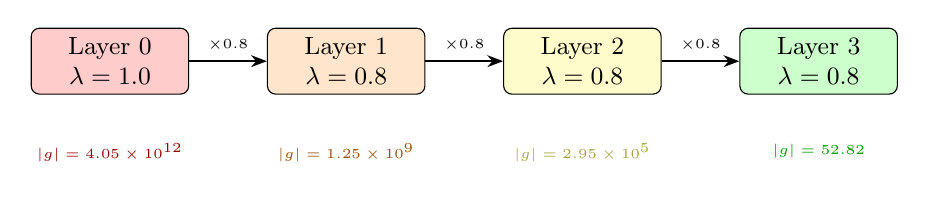
\begin{tikzpicture}[
    layer/.style={rectangle, draw, rounded corners=3pt, minimum height=0.8cm, minimum width=2cm, align=center, font=\small},
    arrow/.style={-{Stealth[length=2mm]}, thick}
]

\node[layer, fill=red!20] (l0) at (0, 0) {Layer 0\\$\lambda=1.0$};
\node[layer, fill=orange!20] (l1) at (3, 0) {Layer 1\\$\lambda=0.8$};
\node[layer, fill=yellow!20] (l2) at (6, 0) {Layer 2\\$\lambda=0.8$};
\node[layer, fill=green!20] (l3) at (9, 0) {Layer 3\\$\lambda=0.8$};

\draw[arrow] (l0) -- (l1) node[midway, above, font=\tiny] {$\times 0.8$};
\draw[arrow] (l1) -- (l2) node[midway, above, font=\tiny] {$\times 0.8$};
\draw[arrow] (l2) -- (l3) node[midway, above, font=\tiny] {$\times 0.8$};

\node[below=0.5cm of l0, font=\tiny, text=red!60!black] {$|g| = 4.05 \times 10^{12}$};
\node[below=0.5cm of l1, font=\tiny, text=orange!60!black] {$|g| = 1.25 \times 10^{9}$};
\node[below=0.5cm of l2, font=\tiny, text=yellow!60!black] {$|g| = 2.95 \times 10^{5}$};
\node[below=0.5cm of l3, font=\tiny, text=green!60!black] {$|g| = 52.82$};

\end{tikzpicture}
\caption{Progressive layer decay: gradient magnitudes decrease exponentially across layers.}
\label{fig:layer-decay}
\end{figure}

The progressive decay ensures that while shallow layers experience large gradients (enabling rapid feature learning), deeper layers remain stable (preventing divergence in the output).

\subsubsection{Mechanism 3: Energy Conservation}

Physical operators in the Spacetime Engine satisfy energy conservation:
\begin{equation}
\|F\|_{\text{energy}} = \text{constant after normalization}
\end{equation}

Energy normalization (Section 6 of~\cite{lsh-sfa}) rescales the field after each PDE step, preventing unbounded growth even when individual gradient components are large.

\subsection{V2 Stateless Gradient Architecture}

Based on the three principles of the LSH semantic architecture~\cite{lsh-three-layer}:

\begin{enumerate}
\item \textbf{Elements store body, not changes}: Field values are primary; gradients are derived
\item \textbf{Gradients are relations, not properties}: Gradients describe relationships between fields, not stored attributes
\item \textbf{History is traced back, not stored}: Gradient computation is stateless; no gradient accumulation buffer
\end{enumerate}

\begin{table}[h]
\centering
\caption{V1 vs V2 gradient architecture.}
\label{tab:v1v2}
\begin{tabular}{lcc}
\toprule
\textbf{Aspect} & \textbf{V1} & \textbf{V2} \\
\midrule
Structure & field\_value + grad\_field & field\_value only \\
Rule & perception\_rule & GradientRule \\
Execution & Store gradients & Return gradients \\
Memory & O(n) & O(1) \\
\bottomrule
\end{tabular}
\end{table}

\subsection{Experiments}

\begin{table}[h]
\centering
\caption{Training results comparison.}
\label{tab:results}
\begin{tabular}{lcc}
\toprule
\textbf{Method} & \textbf{Loss Reduction} \\
\midrule
Pure Autograd & 42.7\% \\
V2 Gradient & 46.1\% \\
\bottomrule
\end{tabular}
\end{table}

\section{Discussion: Encoding and Gradient are Connected}

The collapse phenomenon (Part I) and controllable explosion (Part II) are two sides of the same coin. Both arise from the interaction between encoding granularity and gradient dynamics:

\begin{itemize}
\item \textbf{Fine-grained encoding} (UTF-8 bytes, 256 classes) creates large output gradients that can overwhelm shallow layers, leading to collapse without pretraining
\item \textbf{Physical priors} (conjugate Laplacian, energy normalization) provide gradient direction alignment that prevents divergence even when magnitudes are large
\item \textbf{Unicode BMP} (65,536 classes) increases output dimensionality but reduces sequence length, shifting the gradient burden from temporal to spatial dimensions
\end{itemize}

This suggests that future tokenizer-free models should co-design the encoding scheme and gradient management strategy.

\section{Conclusion}

We have analyzed two aspects of training dynamics in physics-informed neural networks:

\begin{enumerate}
\item \textbf{Tokenizer-Free Encoding}: Unicode BMP provides optimal balance for tokenizer-free Chinese modeling (1x sequence length, 65,536 vocabulary). The collapse phenomenon is a shared limitation of fine-grained classification without pretraining, not an architecture-specific defect.
\item \textbf{Controllable Explosion}: Gradient magnitude explosion in LSH-SFA is controllable through conjugate Laplacian alignment, progressive layer decay, and energy conservation. The V2 stateless gradient architecture achieves 46.1\% loss reduction.
\end{enumerate}

Future work includes developing pretraining strategies for Unicode BMP models and formalizing the connection between encoding granularity and gradient stability.

\section{Validation Roadmap}

\subsection{Collapse Theory (Short-Term)}

\begin{enumerate}
\item \textbf{Gradient vanishing analysis}: Trace gradient norms through each layer during collapse training to determine whether collapse is caused by vanishing gradients (output layer) or gradient conflict (competing classification vs.\ representation objectives)
\item \textbf{Representation degeneration}: Analyze the rank of hidden state matrices during collapse to test the hypothesis that fine-grained output classification causes representation collapse to a low-rank subspace
\item \textbf{Pretraining mitigation}: Train Unicode BMP models with pretrained byte-level embeddings (transferred from a UTF-8 byte model) to test whether pretraining eliminates collapse
\end{enumerate}

\subsection{Controllable Explosion Formalization (Medium-Term)}

\begin{enumerate}
\item \textbf{Convergence proof}: Prove that under the conditions of conjugate Laplacian alignment, progressive layer decay ($\lambda_l < 1$), and energy normalization, the training dynamics converge despite gradient magnitude explosion. Formally, show that $\lim_{t \to \infty} \mathcal{L}(\theta_t) < \infty$ even when $\|\nabla_\theta \mathcal{L}\| \to \infty$
\item \textbf{Lyapunov stability}: Construct a Lyapunov function $V(\theta) = \mathcal{L}(\theta) + \lambda \|F\|_{\text{energy}}^2$ and show that $dV/dt < 0$ along training trajectories, proving that energy normalization acts as a Lyapunov stabilizer
\item \textbf{Optimal decay schedule}: Determine the optimal progressive decay schedule $\lambda_l$ through sensitivity analysis, replacing the current heuristic ($1.0 \rightarrow 0.8 \rightarrow 0.8 \rightarrow 0.8$) with a principled schedule
\end{enumerate}

\subsection{Encoding-Gradient Co-Design (Long-Term)}

\begin{enumerate}
\item \textbf{Joint optimization}: Develop a theoretical framework that co-optimizes encoding vocabulary size and gradient management strategy, deriving the optimal vocabulary size as a function of model depth and width
\item \textbf{Cross-lingual validation}: Test Unicode BMP encoding on multilingual benchmarks (Chinese, Japanese, Korean, Arabic) to validate the 3x sequence length reduction claim across language families
\end{enumerate}

\bibliographystyle{plainnat}
\begin{thebibliography}{10}

\bibitem[Baydin et~al.(2018)]{baydin2018automatic}
Atilim~Gunes Baydin, Barak~A Pearlmutter, Alexey~Andreyevich Radul, and Jeffrey Mark Siskind.
\newblock Automatic differentiation in machine learning: A survey.
\newblock \emph{Journal of Machine Learning Research}, 18:1--43, 2018.

\bibitem[Li(2026a)]{lsh-sfa}
Hengbo Li.
\newblock LSH-SFA: Spacetime Field Attention with Wave Packets, Light-Cone Causality, and PDE-Driven Evolution.
\newblock \emph{LSH Protocol Preprint}, 2026.

\bibitem[Li(2026b)]{lsh-three-layer}
Hengbo Li.
\newblock LSH: Element-Observers Semantic Architecture with Emergent Execution.
\newblock \emph{LSH Protocol Preprint}, 2026.

\bibitem[Sennrich et~al.(2016)]{sennrich2016neural}
Rico Sennrich, Barry Haddow, and Alexandra Birch.
\newblock Neural machine translation of rare words with subword units.
\newblock In \emph{ACL}, 2016.

\bibitem[Vaswani et~al.(2017)]{vaswani2017attention}
Ashish Vaswani, Noam Shazeer, Niki Parmar, Jakob Uszkoreit, Llion Jones, Aidan~N Gomez, {\L}ukasz Kaiser, and Illia Polosukhin.
\newblock Attention is all you need.
\newblock In \emph{NeurIPS}, 2017.

\end{thebibliography}

\end{document}
